\documentclass{article}

\usepackage{amsmath}
\usepackage{amssymb}
\usepackage{hyperref}
\usepackage{url}
\usepackage{graphicx}
\usepackage{geometry}
\usepackage{enumitem}
\usepackage{parskip}
\usepackage{chemfig}
\usepackage{pdfpages}
\usepackage{xcolor}
\usepackage{tikz}
\usepackage{fancybox}
\usepackage{makecell}
\usepackage{pgfplots}
\usepackage{soul}
\usepackage{ulem}
\usepackage{wrapfig}
\usepackage{subcaption}
\usepackage[T1]{fontenc}
\usepackage{esvect}
\usepackage{multirow}
\usepackage{booktabs}
\usepackage{float}
\usepackage{tocloft}
\usepackage{caption}
\usepackage{colortbl}
\usetikzlibrary{arrows}
\usetikzlibrary{decorations.pathreplacing}
\pgfplotsset{compat=1.17}
\usepgfplotslibrary{statistics}
\definecolor{darkgray}{rgb}{0.2, 0.2, 0.2}

% === BIBLIOGRAPHY ===
\usepackage[utf8]{inputenc}
\usepackage{csquotes}
\usepackage[style=apa, backend=biber, doi=true, url=true]{biblatex}
\addbibresource{ref.bib}
\DeclareFieldFormat[article]{volume}{\textbf{#1}}
\DeclareFieldFormat[article]{journaltitle}{\textit{#1}}
% ====================
 
\geometry{
    a4paper,
    total={170mm, 257mm},
    left=20mm,
    top=20mm
}

\hypersetup{
    colorlinks=true,
    linkcolor=black,
    urlcolor=blue,
    pdftitle={Report SW10 - EnCheBio}
}

\newcommand{\figbox}[1]{ 
    \begin{figure*}[ht!]        
        \begin{center}            
            \fbox{#1}        
        \end{center}    
    \end{figure*}
}

\newcommand{\wrapfill}{
    \par
    \ifnum \value{WF@wrappedlines} > 0
        \addtocounter{WF@wrappedlines}{-1}%
        \null\vspace{
            \arabic{WF@wrappedlines}
            \baselineskip
        }
        \WFclear
    \fi
    \phantom{}
}

\newcommand{\cfig}[1]{%
  \begin{figure*}[ht!]%
    \centering%
    #1%
  \end{figure*}%
}

% === LIST OF EQUATIONS ===
\newcounter{myequation}
\renewcommand{\themyequation}{\arabic{myequation}}

\newlistof{myequations}{loe}{\Large List of Equations}
\newcommand{\addequationtotoc}[1]{\addcontentsline{loe}{myequations}{\protect\numberline{\themyequation}#1}}

\renewcommand{\cftmyequationspresnum}{}
\renewcommand{\cftmyequationsaftersnum}{\hspace{1em}}
\setlength{\cftmyequationsnumwidth}{2em}
\cftsetindents{myequations}{1.5em}{2.3em}

\newcommand{\capeq}[3]{
    \refstepcounter{myequation}
    \begin{equation*}
        #1
    \end{equation*}
    \label{#2}
    \begin{center}
        \vspace*{-.4cm}
        \noindent{Equation \themyequation:} #3
    \end{center}
    \addequationtotoc{#3}
}

\newcommand{\refeq}[1]{\hyperref[#1]{[Equation~\ref*{#1}]}}
% =========================

\newcommand{\difference}{\,\backslash\,}
\newcommand{\rem}{\underline{Remark}: }
\newcommand{\nots}{\underline{Notation}: }
\newcommand{\prf}{\underline{Proof}: }
\newcommand{\exs}{\underline{Example}: }
\newcommand{\defs}{\underline{Definition}: }
\newcommand{\wrn}{\underline{Warning}: }
\newcommand{\sht}{\ |\ }
\newcommand{\pph}[1]{\paragraph{#1}\phantom{}\\}

% === TEXT ===
\begin{document}

\hypersetup{citecolor=black}

\begin{minipage}{0.7\textwidth}
    \vspace*{-.8cm} \hspace*{-0.3cm}
    
\includegraphics[width=.5\textwidth]{media/hslu-logo.png}
\end{minipage}

\vspace*{2cm}

\textbf{\huge Practical 2:}\\[.75cm]
\begin{center}
    \textbf{\huge Water Hardness: Chemistry,}
    
    \textbf{\huge Measurement, and Effects}\\[1cm]
    
    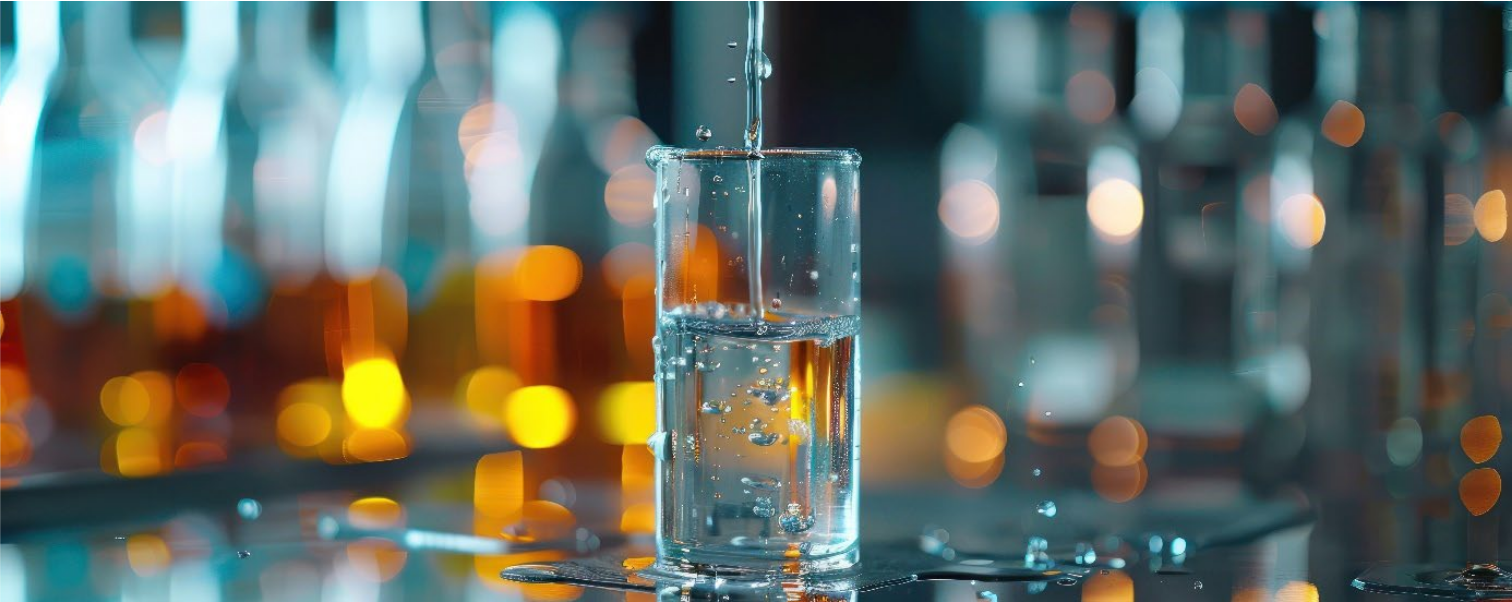
\includegraphics[width=\textwidth]{media/front_practical2.png}\\
\end{center}

\vfill

\setlength{\intextsep}{0pt}%
\begin{wrapfigure}{r}{\textwidth}
    \textbf{\Large Environmental Chemistry and Biology HS2024\\[.5cm]
    \large Dr. Macarena San Martín Ruiz\\
    Lecturer}
    \vspace{-2.1cm}
\end{wrapfigure}

\phantom{}\\[-1cm]

\begin{flushright}
        \large
        \textbf{Team 4}\\
        Matteo Frongillo\\
        Ramadhan Nura\\
        Folagbade Popoola\\
        Jonathan Lawrence Boms\\
        Kron Xhemajli
\end{flushright}
\wrapfill

\tableofcontents
\pagebreak

\section{Introduction}
Water hardness is an essential parameter that reflects the concentration of calcium (\(\text{Ca}^{2+}\)) and magnesium (\(\text{Mg}^{2+}\)) ions in water. It significantly influences daily activities, such as washing and cooking, as well as industrial operations that rely on water as a key resource. 

This experiment focuses on comparing the hardness of two water sources (tap water and bottled water). The titration method, using EDTA as a chelating agent, was employed to quantify water hardness. Additionally, pH measurements were used to assess the chemical behavior of both water types during the titration process.

By analyzing the collected data and interpreting the results through graphical and statistical methods, the study aims to highlight the differences between the two water sources, their practical implications, and their potential impact on household, industrial, and health-related applications.

\subsection{Water hardness}
Water hardness is a critical parameter that affects numerous daily activities, from washing
clothes and dishes to industrial processes and agricultural practices. Understanding the
hardness of water is essential for optimizing soap usage, preventing scale formation in
pipes and boilers, and ensuring the efficient operation of various water-using appliances

\vspace*{.5cm}
\begin{table}[h!]
    \centering
    \caption{Classification of water hardness}
    \begin{tabular}{@{}lclcl@{}}
    \toprule
    \textbf{$^\circ$fH} & & \textbf{mmol/L} & & \textbf{Hardness}\\
    \midrule
    0 -- 7 & & 0 -- 0.7 & & Very soft\\ 
    7 -- 15 & & 0.7 -- 1.5 & & Soft\\ 
    15 -- 25 & & 1.5 -- 2.5 & & Moderately hard\\ 
    25 -- 32 & & 2.5 -- 3.2 & & Fairly hard\\ 
    32 -- 42 & & 3.2 -- 4.2 & & Hard\\ 
    $\leq$ 42 & & $\leq$ 4.2 & & Very hard\\
    \bottomrule
    \end{tabular}
    \label{tab:water-hardness}
\end{table}

\section{Materials and methods}
\subsection{List of materials}
\begin{minipage}[t]{0.48\textwidth}
\begin{itemize}
    \item Water sample (bottled water and tap water)
    \item 0.01[M] EDTA solution (standard solution)
    \item Indicator buffer tablets (Ammonia tablets)
    \item Pipette (10 mL)
    \item Burette (25 mL)
    \item Conical flask (100 mL)
\end{itemize}
\end{minipage}%
\hfill
\begin{minipage}[t]{0.48\textwidth}
\begin{itemize}
    \item Distilled water
    \item White tile (to observe the color change)
    \item Magnetic stirrer
    \item Stick to mix
    \item 8 flasks of 100 ml
    \item pH meter
\end{itemize}
\end{minipage}

\subsection{Procedure}\label{sub:procedure}
At the beginning of the lab process, we measured 75 ml of tap water
and filled 3 beakers with the same volume. Indicator buffer tablets
(Ammonia [NH$_3$] tablets) were then added to the beakers with water and
mixed until they dissolved. A volume of 50 ml of EDTA solution was
then inserted into the burette, and the presence of air bubbles was
checked to prevent errors in the titration process.

To begin the titration, we ensured that everything was set up correctly.
We prepared tables to note down our readings, a white tile to observe
the color change, a magnetic stirrer to mix during titration, and a
pH reader to measure the pH level at regular intervals
(normally after each 1 ml).

With everything set up, we began letting the EDTA solution into the
ammonia and water mixture in drops to achieve precise readings. We
observed the color changes as well as recorded the pH level at
regular intervals to determine when the endpoint of the titration was
reached.

The experiment was also repeated with a bottled water and ammonia
solution following the same process. The initial pH level was
measured, and the color change during the titration was monitored as
EDTA solution was gradually added. The goal was to record the changes
in color and pH at different stages.

The data collected during the experiments would later be used to
determine the water hardness for each test and to evaluate it through
statistical analysis. Care was taken to avoid parallax error to
ensure accurate measurements.

\newpage
\subsection{Pictures of proceedings}
\begin{minipage}[t]{\textwidth}
    \begin{minipage}[t]{0.29\textwidth}
        \centering
        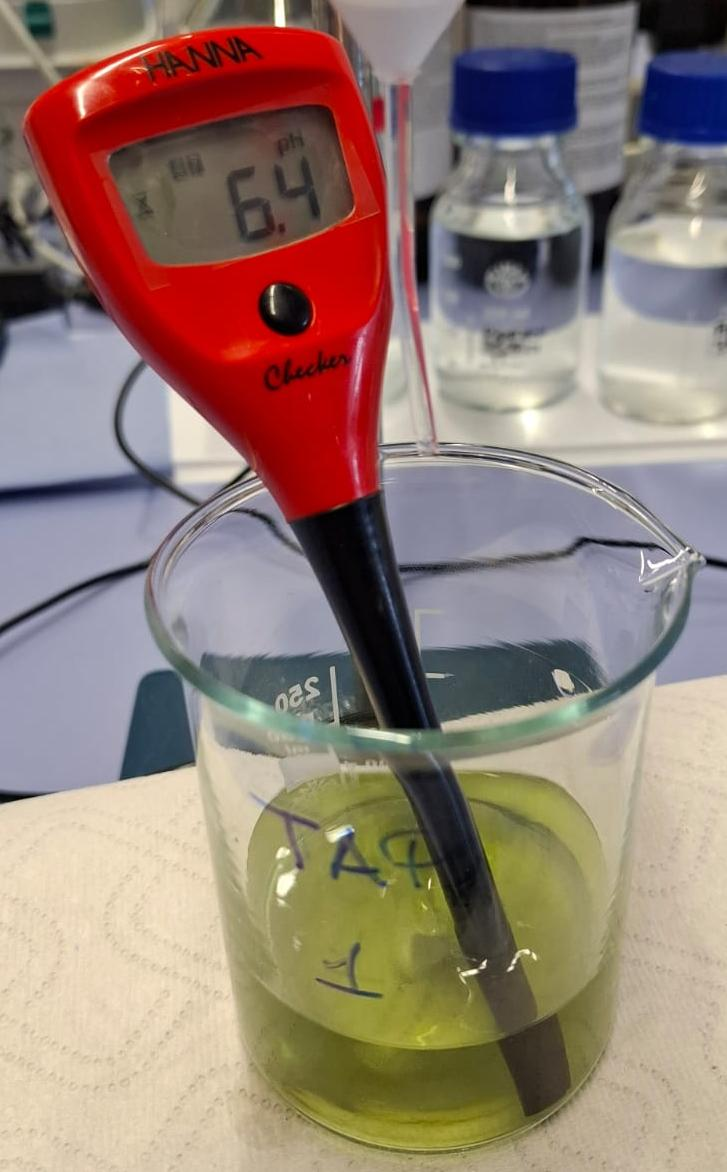
\includegraphics[width=\textwidth]{media/ph-measuring.jpeg}
        \captionof{figure}{pH measurement}
        \label{fig:ph_measuring}
    \end{minipage}
    \hfill
    \begin{minipage}[t]{0.36\textwidth}
        \centering
        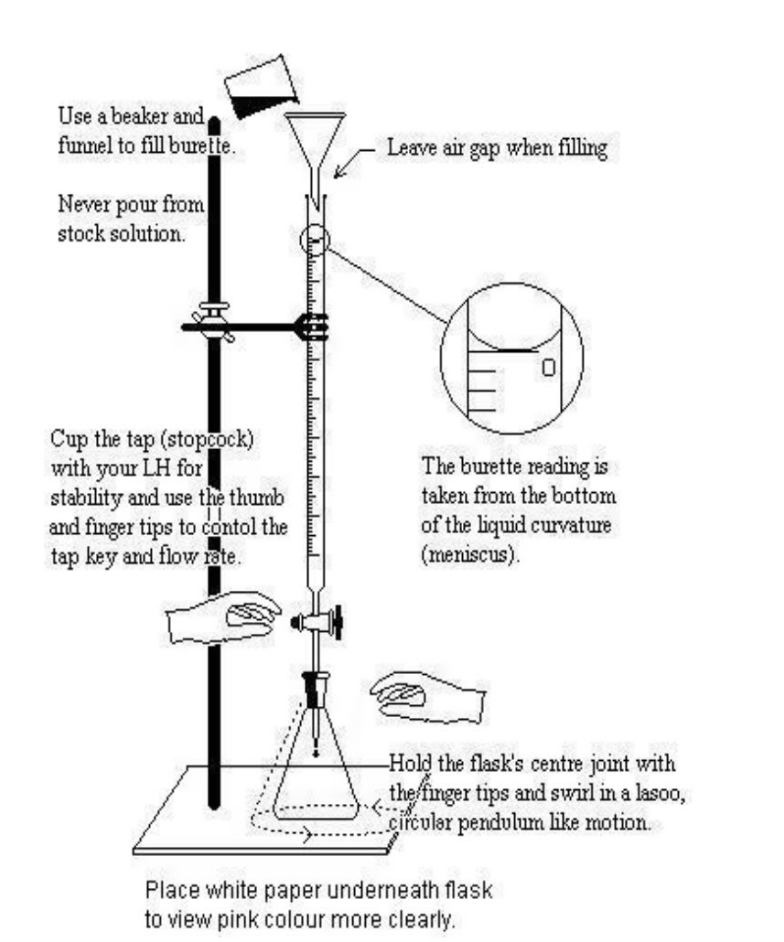
\includegraphics[width=\textwidth]{media/titration_steps.png}
        \captionof{figure}{Titration procedure}
        \label{fig:titration_procedure}
    \end{minipage}
    \hfill
    \begin{minipage}[t]{0.28\textwidth}
        \centering
        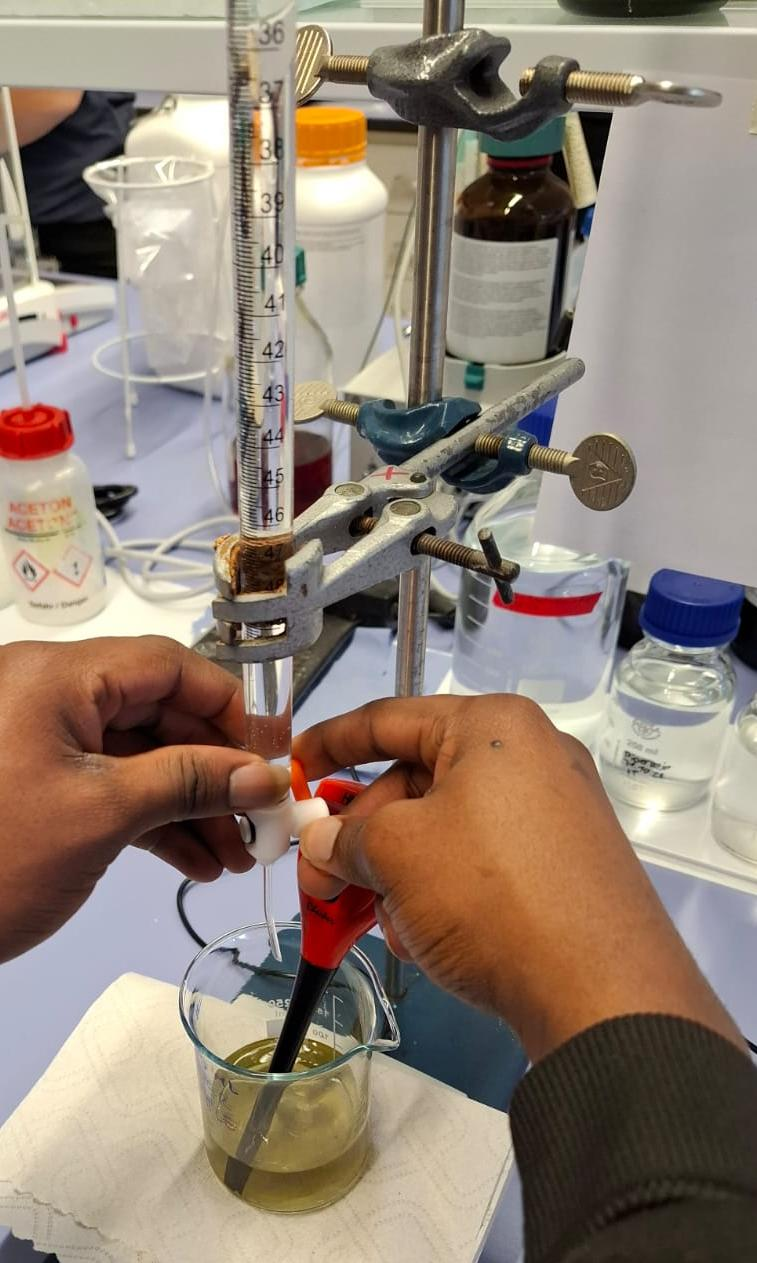
\includegraphics[width=\textwidth]{media/tetration-process.jpeg}
        \captionof{figure}{Moment of titration}
        \label{fig:moment_titration}
    \end{minipage}
\end{minipage}

\vspace{0.7cm}

\begin{minipage}[t]{\textwidth}
    \centering
    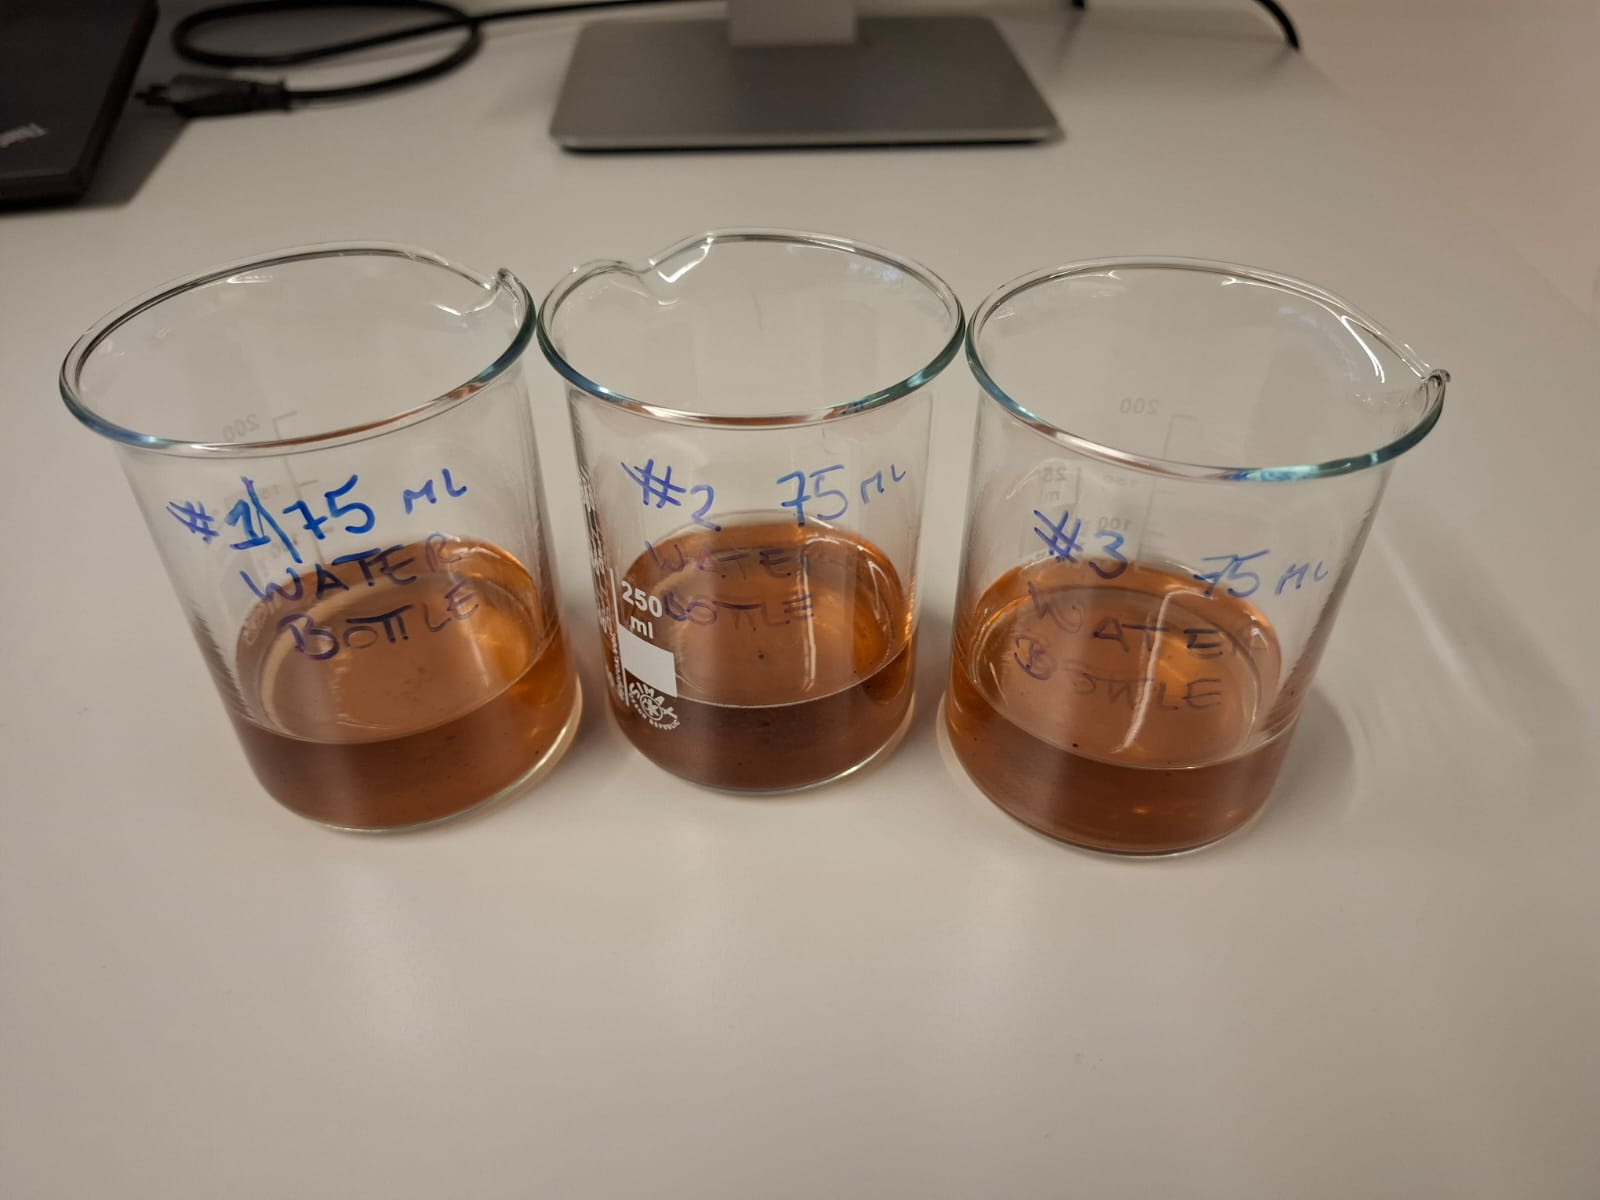
\includegraphics[width=0.6\textwidth]{media/tap-with-ammonia.jpeg}
    \captionof{figure}{Solution of tap water and ammonia}
    \label{fig:solution_tap_ammonia}
\end{minipage}

\section{Results}
\subsection{Experiment parameters}
The parameters of the experiment provide an overview of what data were useful so that
water hardness could be calculated.

\subsubsection{Initial values}
The initial values of water and ammonia samples, at 0 mL EDTA, are as follows:
\vspace*{.3cm}
\begin{table}[h!]
    \caption{Initial values}
    \centering
        \begin{tabular}{@{}lccccc@{}}
            \toprule
            \textbf{Type} & \textbf{mL} & \textbf{pH Sample 1} & \textbf{pH Sample 2} & \textbf{pH Sample 3} & \textbf{pH Average}\\ \midrule
            Tap & 0 & 7.0 & 7.1 & 7.0 & 7.03\\
            Bottled & 0 & 7.4 & 7.5 & N.D. & 7.45\\ \bottomrule
        \end{tabular}
    \label{tab:initial-values}
\end{table}

\subsubsection{Titration parameters}
Measurements were made on two different types of water (tap and bottle) three times each,
and then the initial and final parameters of each sample were marked so that the water
hardness for each milliliter of EDTA could be easily calculated.

\subsubsection{pH parameters}
Just as the parameters were computed for the titration calculation, pH measurements were
also made under the same circumstances. Having known the amount of EDTA poured into the
solution of water and ammonia, it was possible to correctly identify the amount of solvent
needed to allow the fluid to change color, consequently facilitating the calculation of
water hardness.

\subsection{Formulas}
\subsubsection{Water hardness}
The formula for calculating water hardness, expressed in $^\circ$fH, takes into account the
volume of water inside the beaker, the molarity of the EDTA solution and its volume used,
and finally the total volume of the sample:
\capeq{\text{Hardness (mg/L CaCO}_3) = \frac{M_{\text{EDTA}} \times V_{\text{EDTA}} \times 1000 \times 100}{V_{\text{sample}}}}{eq:water_hardness}{Water hardness}

\subsubsection{Mean}
Tables to be completed require calculating an average value of repeated experiments on the
same type of water. For this, the following formula is used:
\capeq{\overline{x} = \frac{1}{n} \sum_{i=1}^{n} x_i}{eq:mean}{Arithmetic mean formula}

\subsubsection{pH drop}
To enhance the graphical visualization of pH variations, the average pH values were
transformed
using the following formula:
\capeq{T(\text{pH}) = \exp(\text{pH} - 7)}{eq:exp-ph}{pH drop formula}

\subsection{Visible results}
The results image shows the final colorations of the samples after titration.
The yellow exhausted color is clearly visible.
\vspace*{.5cm}
\cfig{
    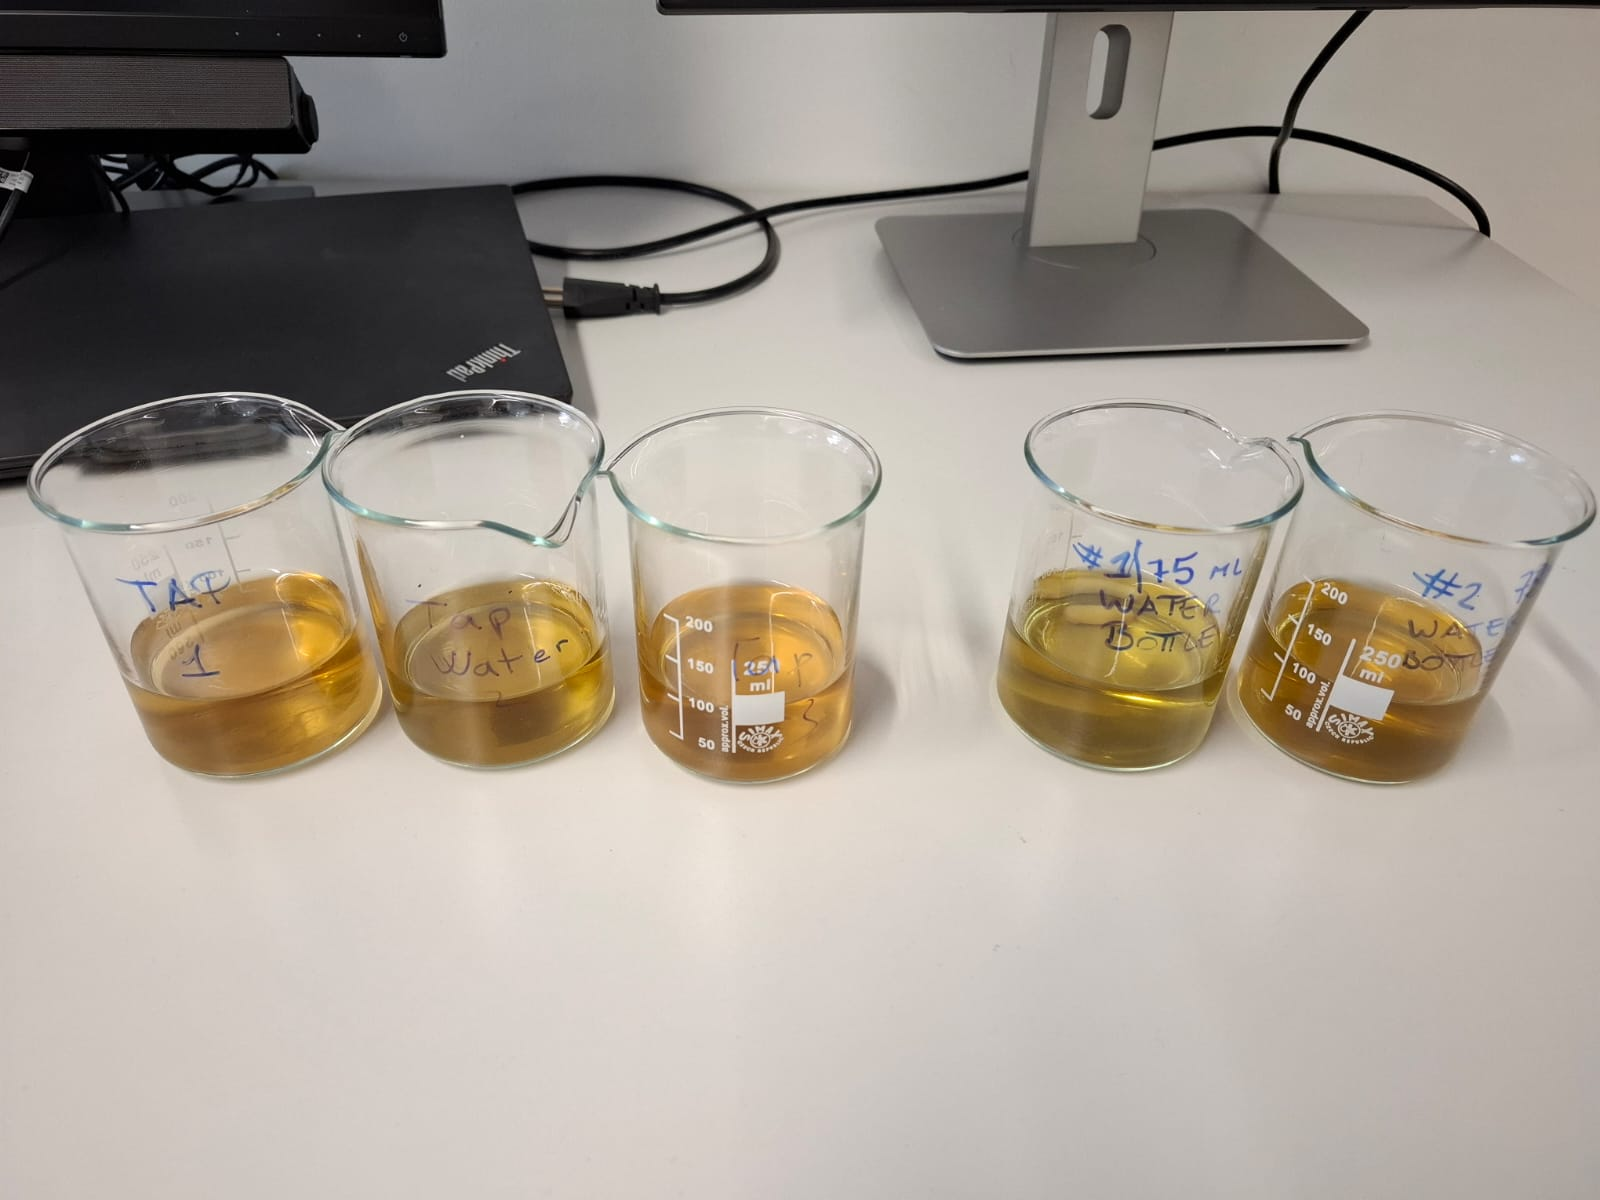
\includegraphics[width=.8\textwidth]{media/final-results.jpeg}
    \label{fig:final-results}
    \caption{Beakers with final solutions}
}

\newpage
\subsection{pH results}\label{sub:pH_results}
\subsubsection{Tap water}
The experiment with tap water was conducted up to 15mL EDTA until the desired final color (dirty yellow) was achieved, which generally indicates the end of the test.
The final results were then recorded:
\vspace*{.5cm}
\renewcommand{\arraystretch}{1.2}
\begin{table}[h!]
    \caption{Tap water pH measurements}
    \centering
    \begin{tabular}{@{}cccccc@{}}
        \toprule
        \textbf{mL} & \textbf{pH Sample 1} & \textbf{pH Sample 2} & \textbf{pH Sample 3} & \textbf{pH Average} & \textbf{T(\text{pH})}\\ \midrule
        0  & 7.0 & 7.1 & 7.0 & 7.03 & 1.03\\
        1  & 7.0 & 7.0 & 7.0 & 7.00 & 1.00\\
        2  & 6.8 & 6.8 & 6.8 & 6.80 & 0.819\\
        3  & 6.7 & 6.6 & 6.6 & 6.63 & 0.691\\
        4  & 6.5 & 6.6 & 6.5 & 6.55 & 0.638\\
        5  & 6.5 & 6.4 & 6.3 & 6.40 & 0.549\\
        6  & 6.3 & 6.1 & 6.1 & 6.17 & 0.436\\
        7  & 6.1 & 5.8 & 5.9 & 5.93 & 0.343\\
        8  & 6.0 & 5.6 & 5.7 & 5.77 & 0.292\\
        9  & 5.8 & 5.5 & 5.5 & 5.60 & 0.247\\
        10 & 5.6 & 5.4 & 5.5 & 5.50 & 0.223\\
        11 & 5.4 & 5.4 & 5.4 & 5.40 & 0.202\\
        12 & 5.4 & 5.3 & 5.3 & 5.33 & 0.188\\
        13 & 5.3 & 5.3 & 5.3 & 5.30 & 0.183\\
        14 & 5.3 & 5.3 & 5.3 & 5.30 & 0.183\\
        15 & 5.3 & 5.3 & 5.2 & 5.27 & 0.177\\ \bottomrule
    \end{tabular}
    \label{tab:ph-measurements}
\end{table}
\pph{Graphical rappresentation}
\begin{figure}[h!]
    \centering
    \begin{tikzpicture}
    \begin{semilogxaxis}[
        width=0.9\textwidth,
        height=0.5\textwidth,
        xlabel={mL (log scale)},
        ylabel={pH drop},
        ymin=0, ymax=1.2,
        xmin=0.075, xmax=20,
        grid=major,
        legend pos=south west,
        legend style={font=\small},
        legend cell align={left},
    ]

    \addplot[
        domain=0.1:15,
        samples=500,
        thick,
        color=black
    ] {1.05345 * exp(-0.1624 * x) + 0.0434};
    \addlegendentry{$y = 1.05e^{-0.16x} + 0.04$}

    \addplot[only marks, mark=*, color=blue] coordinates {
        (0.1,1.0305) (1,1.0000) (2,0.8187) (3,0.6907) (4,0.6376)
        (5,0.5488) (6,0.4360) (7,0.3430) (8,0.2923) (9,0.2466) 
        (10,0.2231) (11,0.2019) (12,0.1882) (13,0.1827) (14,0.1827) (15,0.1773)        
    };
    \addlegendentry{Data points}
    
    \addplot[
        only marks,
        mark=*,
        mark options={color=red},
    ] coordinates {(6.5, 0.411127416057)};
    \node[above right] at (axis cs:6.5, 0.411127416057) {$I_1(6.5, 0.41)$};
    \addlegendentry{Log inflection point}
    
    \end{semilogxaxis}
    \end{tikzpicture}
    \caption{Graph of pH drop for tap water}
    \label{fig:tap_ph}
\end{figure}
\vspace*{.25cm}

The graph, given by the function $y = 1.05e^{-0.16x} + 0.04$,
shows an exponential decrease $T$(pH) as EDTA is added.

The logarithmic scale for volume highlights the gradual decrease at
low levels of EDTA and the inflection point ($I_1$), where the solvent's color
changes noticeably.
Initially, the pH decreases slightly (from 7.0 to 6.8), as the amount of EDTA is
insufficient to fully bind the hardness ions. With more EDTA, the pH
drops more significantly.

\subsubsection{Bottled water}
The experiment with bottled water was conducted up to 25mL EDTA. The pH values were measured for two samples, and their average was calculated as shown below:
\vspace*{.5cm}
\renewcommand{\arraystretch}{1.2}
\begin{table}[h!]
    \caption{Bottled water pH measurements}
    \hspace*{-1.5cm}
    \begin{minipage}[t]{0.45\textwidth}
        \centering
        \caption*{(0 -- 13 mL)}
        \begin{tabular}{@{}ccccc@{}}
            \toprule
            \textbf{mL} & \textbf{pH Sample 1} & \textbf{pH Sample 2} & \textbf{pH Average} & \textbf{T(pH)}\\ \midrule
            0  & 7.4 & 7.5 & 7.45 & 1.568\\
            1  & 7.3 & 7.4 & 7.35 & 1.419\\
            2  & 7.2 & 7.3 & 7.25 & 1.284\\
            3  & 7.2 & 7.3 & 7.25 & 1.284\\
            4  & 7.1 & 7.2 & 7.15 & 1.162\\
            5  & 7.0 & 7.1 & 7.05 & 1.051\\
            6  & 7.0 & 7.0 & 7.00 & 1.000\\
            7  & 7.0 & 6.9 & 6.95 & 0.951\\
            8  & 6.9 & 6.8 & 6.85 & 0.861\\
            9  & 6.9 & 6.7 & 6.80 & 0.819\\
            10 & 6.8 & 6.65 & 6.73 & 0.763\\
            11 & 6.7 & 6.6 & 6.65 & 0.705\\
            12 & 6.7 & 6.55 & 6.63 & 0.691\\
            \bottomrule
        \end{tabular}
    \end{minipage}
    \hfill
    \begin{minipage}[t]{0.45\textwidth}
        \centering
        \caption*{(14 -- 25 mL)}
        \begin{tabular}{@{}cccc@{}}
            \toprule
            \textbf{pH Sample 1} & \textbf{pH Sample 2} & \textbf{pH Average} & \textbf{T(pH)}\\ \midrule
            6.6 & 6.5 & 6.55 & 0.638\\
            6.5 & 6.4 & 6.45 & 0.577\\
            6.5 & 6.3 & 6.40 & 0.549\\
            6.4 & 6.2 & 6.30 & 0.497\\
            6.3 & 6.2 & 6.25 & 0.472\\
            6.2 & 6.1 & 6.15 & 0.427\\
            6.1 & 5.9 & 6.00 & 0.368\\
            6.1 & 5.9 & 6.00 & 0.368\\
            6.0 & 5.8 & 5.90 & 0.333\\
            5.9 & 5.7 & 5.80 & 0.301\\
            5.8 & 5.7 & 5.75 & 0.287\\
            5.8 & 5.6 & 5.70 & 0.273\\
            5.7 & 5.6 & 5.65 & 0.259\\
            \bottomrule
        \end{tabular}
    \end{minipage}
    \label{tab:ph-measurements-bottled}
\end{table}
\vspace*{.25cm}

\pph{Graphical representation}
\begin{figure}[h!]
    \centering
    \begin{tikzpicture}
    \begin{semilogxaxis}[
        width=0.9\textwidth,
        height=0.5\textwidth,
        xlabel={mL (log scale)},
        ylabel={pH drop},
        ymin=0, ymax=1.5,
        xmin=0.9, xmax=30,
        grid=major,
        legend pos=south west,
        legend style={font=\small},
        legend cell align={left},
    ]

    \addplot[
        domain=1:25,
        samples=500,
        thick,
        color=black
    ] {1.58 * exp(-0.07 * x) - 0.05};
    \addlegendentry{$y= 1.58e^{-0.07x} - 0.05$}

    \addplot[only marks, mark=*, color=blue] coordinates {
        (0,1.5683) (1,1.4191) (2,1.2840) (3,1.2840) (4,1.1618) 
        (5,1.0513) (6,1.0000) (7,0.9512) (8,0.8607) (9,0.8187) 
        (10,0.7634) (11,0.7047) (12,0.6907) (13,0.6376) (14,0.5769) 
        (15,0.5488) (16,0.4966) (17,0.4724) (18,0.4274) (19,0.3679) 
        (20,0.3679) (21,0.3329) (22,0.3012) (23,0.2865) (24,0.2725) 
        (25,0.2592)        
    };
    \addlegendentry{Data points}

    \addplot[
        only marks,
        mark=*,
        mark options={color=red},
    ] coordinates {(19, 0.367874072854)};
    \node[below left] at (axis cs:19, 0.367874072854) {$I_2(19, 0.37)$};
    \addlegendentry{Log inflection point}

    \end{semilogxaxis}
    \end{tikzpicture}
    \caption{Graph of pH drop for bottled water}
    \label{fig:bottled_ph}
\end{figure}
\vspace*{.25cm}

The graph, given by the function $y = 1.58e^{-0.07x} - 0.05$,
as per the intuition given by the experiment done previously, also shows an exponential
decrease in $T$(pH) with the addition of EDTA.

The logarithmic scale for volume was used again to show the gradual decrease at EDTA
levels and the inflection point ($I_2$), where the color of the solvent changes noticeably.
In this experiment, the pH has a more abrupt change around an amount of
19mL EDTA poured into the solution of bottled water and ammonia.

\newpage
\section{Water hardness results}
\subsection{Legend and formulas}
\subsubsection{Legend}
\begin{itemize}
    \item \textbf{ID}: Sample number of the water solution
    \item $\mathbf{V_{s,i}}$: Initial volume of the water sample (mL)
    \item $\mathbf{V_{b,i}}$: Initial volume of EDTA inside the burette (mL)
    \item $\mathbf{V_{b,f}}$: Final volume of EDTA inside the burette (mL)
    \item $\mathbf{\Delta V}$: Volume of EDTA used (mL)
    \item $\mathbf{V_{s,f}}$: Final volume of the water and EDTA sample (mL)
\end{itemize}

\subsubsection{Formulas}
The following formulas were used to complete the tables and to calculate water hardness:
\begin{itemize}
    \item \textbf{Volume of EDTA used}
        \capeq{\Delta V = V_{b,f} - V_{b,i}}{eq:V_EDTA}{Volume of EDTA used}
    \item \textbf{Final volume of water + EDTA sample}
    \capeq{V_{s,f} = V_{s,i} + \Delta V}{eq:V_tot}{Total sample volume}
    \item \textbf{Hardness conversion}\\
    The conversion of water hardness from mg/L CaCO$_3$ to $^\circ$fH was done on the basis of \refeq{eq:water_hardness}:
    \capeq{\text{Hardness} \left(^\circ\text{fH}\right) = \text{Hardness (mg/L CaCO}_3) \cdot 10^{-1}\ \phantom{}^\circ\text{fH}\cdot\text{L/mg}}{eq:fH_formula}{Water hardness in $^\circ$fH}
    \item \textbf{Standard deviation}
    \capeq{\sigma = \sqrt{\frac{1}{n-1} \sum_{i=1}^{n} (x_i - \overline{x})^2}}{eq:std}{Standard deviation formula}
\end{itemize}

\subsection{Tap water}
As emphasized in the chapter \ref{sub:procedure}, the following table shows the initial and
final values of the experiment, highlighting at what $\Delta V$ the solution of water and
ammonia changed color. The $\Delta V$ values represent on the graph the logarithmic inflection
points ($I_1, I_2$), previously identified and commented on in the chapter \ref{sub:pH_results}.

\subsubsection{Data set}
\begin{table}[h!]
    \caption{Tap water hardness}
    \centering
    \begin{tabular}{@{}cccccc@{}}
        \toprule
        \textbf{ID} & $\mathbf{V_{s,i}}$ & $\mathbf{V_{b,i}}$ & $\mathbf{V_{b,f}}$ & $\mathbf{\Delta V}$ & $\mathbf{V_{s,f}}$ \\
        \midrule
        Tap 1 & 75 & 50 & 40 & 10 & 85\\ 
        Tap 2 & 75 & 50 & 42 & 8  & 83\\ 
        Tap 3 & 75 & 50 & 43 & 7  & 82\\ 
        \bottomrule
    \end{tabular}
    \label{tab:tap-hardness}
\end{table}

\newpage
\subsubsection{Hardness calculation}
Using the formula \refeq{eq:water_hardness} and \refeq{eq:fH_formula}:
\capeq{\text{Tap 1} \left(^\circ\text{fH}\right) = \frac{0.01 [M] \cdot 10 \text{mL} \cdot 1000 \cdot 100}{10\cdot 85 \text{mL}} \approx 11.76 ^\circ\text{fH}}{eq:tap_hardness_1}{Hardness of Tap 1}

\capeq{\text{Tap 2} \left(^\circ\text{fH}\right) = \frac{0.01 [M] \cdot 8 \text{mL} \cdot 1000 \cdot 100}{10\cdot 83 \text{mL}} \approx 9.64 ^\circ\text{fH}}{eq:tap_hardness_2}{Hardness of Tap 2}

\capeq{\text{Tap 3} \left(^\circ\text{fH}\right) = \frac{0.01 [M] \cdot 7 \text{mL} \cdot 1000 \cdot 100}{10\cdot 83 \text{mL}} \approx 8.54 ^\circ\text{fH}}{eq:tap_hardness_3}{Hardness of Tap 3}

\subsubsection{Statistical analysis}
Using the measured water hardness values, statistical analyses were performed.
The following calculations were carried out:

\pph{Median calculation}
The median is the middle value of the ordered dataset:
\[
\text{Ordered set: } \{8.54^\circ\text{fH}, \, 9.64^\circ\text{fH}, \, 11.76^\circ\text{fH}\}
\]
\[
\text{Median} = 9.64^\circ\text{fH}
\]

\pph{Standard deviation calculation}
According to the formula \refeq{eq:std}:
\capeq{\sigma_{tap} = \sqrt{\frac{(8.54 - 9.98)^2 + (9.64 - 9.98)^2 + (11.76 - 9.98)^2}{3-1}} \approx \sqrt{2.68} \approx 1.64^\circ\text{fH}}{eq_tap_sdt}{Tap water standard deviation}

\pph{Water hardness table}
\begin{table}[h!]
    \caption{Tap water hardness measurements with deviations}
    \centering
    \begin{tabular}{@{}cccc@{}}
        \toprule
        \textbf{Sample} & \textbf{Hardness} & $\mathbf{x_i - \overline{x}}$ \\
        & \textbf{($^\circ$fH)} & \textbf{($^\circ$fH)} \\
        \midrule
        Tap 1 & 11.76 & +1.78 \\
        Tap 2 & 9.64  & -0.34 \\
        Tap 3 & 8.54  & -1.44 \\
        \bottomrule
    \end{tabular}
    \label{tab:tap-water-deviation}
\end{table}

\subsection{Bottled water}
Just as just computed for tap water samples, data will be processed for bottled water samples.

\subsubsection{Data set}
\begin{table}[h!]
    \caption{Bottled water hardness}
    \centering
    \begin{tabular}{@{}cccccc@{}}
        \toprule
        \textbf{ID} & $\mathbf{V_{s,i}}$ & $\mathbf{V_{b,i}}$ & $\mathbf{V_{b,f}}$ & $\mathbf{\Delta V}$ & $\mathbf{V_{s,f}}$ \\
        \midrule
        Bottled 1 & 75 & 50 & 30 & 20 & 95\\ 
        Bottled 2 & 75 & 50 & 32 & 18  & 93\\ 
        \bottomrule
    \end{tabular}
    \label{tab:bottled-hardness}
\end{table}
\vspace*{.25cm}

\subsubsection{Hardness calculation}
Using the formula \refeq{eq:water_hardness} and \refeq{eq:fH_formula}:
\capeq{\text{Bottled 1} \left(^\circ\text{fH}\right) = \frac{0.01 [M] \cdot 20 \text{mL} \cdot 1000 \cdot 100}{10 \cdot 95 \text{mL}} \approx 21.05 ^\circ\text{fH}}{eq:bottled_hardness_1}{Hardness of Bottled 1}

\capeq{\text{Bottled 2} \left(^\circ\text{fH}\right) = \frac{0.01 [M] \cdot 18 \text{mL} \cdot 1000 \cdot 100}{10 \cdot 93 \text{mL}} \approx 19.35 ^\circ\text{fH}}{eq:bottled_hardness_2}{Hardness of Bottled 2}

\subsubsection{Statistical analysis}
Using the measured water hardness values, statistical analyses were performed.
The following calculations were carried out:

\pph{Median calculation}
The median is the middle value of the ordered dataset:
\[
\text{Ordered set: } \{19.35^\circ\text{fH}, \, 21.05^\circ\text{fH}\}
\]
\[
\text{Median} = \frac{19.35 + 21.05}{2} \approx 20.20^\circ\text{fH}
\]

\pph{Standard deviation calculation}
According to the formula \refeq{eq:std}:
\capeq{\sigma_{\text{bottled}} = \sqrt{\frac{(19.35 - 20.20)^2 + (21.05 - 20.20)^2}{2-1}} \approx \sqrt{1.45} \approx 1.20^\circ\text{fH}}{eq_bottled_sdt}{Bottled water standard deviation}

\pph{Water hardness table}
\begin{table}[h!]
    \caption{Bottled water hardness measurements with deviations}
    \centering
    \begin{tabular}{@{}cccc@{}}
        \toprule
        \textbf{Sample} & \textbf{Hardness} & $\mathbf{x_i - \overline{x}}$ \\
        & \textbf{($^\circ$fH)} & \textbf{($^\circ$fH)} \\
        \midrule
        Bottled 1 & 21.05 & +0.85 \\
        Bottled 2 & 19.35 & -0.85 \\
        \bottomrule
    \end{tabular}
    \label{tab:bottled-water-deviation}
\end{table}

\section{Discussion}
The comparison between the tap water and bottled water results highlights significant differences in their chemical composition, specifically in terms of water hardness. These differences are attributable to the source and treatment processes for each type of water.

\subsection{Tap water analysis}
The tap water samples exhibited a lower overall hardness, with values ranging between \(8.54^\circ\text{fH}\) and \(11.76^\circ\text{fH}\). The statistical analysis revealed a median value of \(9.64^\circ\text{fH}\) and a standard deviation of \(1.64^\circ\text{fH}\), indicating a moderate variability among the samples. The lower hardness can be linked to municipal water treatment processes, which often include softening steps to reduce scale formation in pipelines and appliances.

The graph of pH drop for tap water (Figure \ref{fig:tap_ph}) showed a clear exponential decrease as EDTA was added, with a notable inflection point (\(I_1(6.5, 0.41)\)). This point represents the volume of EDTA required to chelate a significant proportion of hardness ions (\(\text{Ca}^{2+}\) and \(\text{Mg}^{2+}\)). The gradual pH decline suggests a relatively low concentration of these ions, consistent with the observed hardness levels.

\subsection{Bottled water analysis}
In contrast, the bottled water samples showed a higher hardness, with values of \(19.35^\circ\text{fH}\) and \(21.05^\circ\text{fH}\). The median hardness was calculated as \(20.20^\circ\text{fH}\), and the standard deviation was \(1.20^\circ\text{fH}\), indicating slightly less variability compared to tap water. The elevated hardness levels suggest that the bottled water source was less treated or derived from a mineral-rich spring, where higher concentrations of \(\text{Ca}^{2+}\) and \(\text{Mg}^{2+}\) are naturally present.

The corresponding pH drop graph (Figure \ref{fig:bottled_ph}) also demonstrated an exponential decline, but with a more abrupt change at the inflection point (\(I_2(19, 0.37)\)). This sharper decrease implies a higher buffering capacity due to the greater presence of hardness ions. The results align with the classification of water hardness, where bottled water falls into the ``moderately hard'' to ``fairly hard'' range.

\subsection{Implications of findings}
The differences in water hardness between tap and bottled water have practical implications. Tap water's lower hardness is advantageous for household and industrial use, minimizing scale formation and reducing soap consumption. However, bottled water's higher mineral content may offer health benefits, as it provides essential minerals like calcium and magnesium. These findings highlight the importance of choosing the appropriate water source based on its intended use.

From a methodological perspective, the use of EDTA titration proved to be a reliable technique for determining water hardness. The precision of measurements, as evidenced by the low standard deviations, underscores the effectiveness of the experimental setup. Additionally, the use of statistical analysis provided a comprehensive understanding of the data distribution and variability.

\subsection{Limitations and future recommendations}
While the experiments yielded accurate results, some limitations should be acknowledged. The small sample size (three tap water samples and two bottled water samples) may not fully represent the variability of each water source. Future studies could include a larger number of samples from diverse locations to enhance the generalizability of the findings.

Moreover, the analysis focused solely on calcium and magnesium ions as contributors to hardness. Investigating the presence of other ions, such as iron or manganese, could provide a more complete picture of water quality. Expanding the scope of the analysis to include other parameters, such as alkalinity and conductivity, would further enrich the understanding of water chemistry.

\subsection{Questions}
\begin{enumerate}
    \item Compare the results of Bottled water vs tap water used for different
        samples. How are the results compared to the water quality from the
        municipality in Horw?

        \textbf{R:\\}
        Bottled water likely shows greater variability in both pH and hardness due to treatment. Tap water, have close pH as the Horw municipality.

        Notable deviations in tap or bottled water from Horw’s baseline may indicate differences in sourcing, treatment, or branding focus.

    \item Based on the Table \ref{tab:water-hardness}, compare your results and discuss.
    
        \textbf{R:\\}
        \textbf{Tap water}:\\
        Aligned closely with Horw’s municipal water but slightly softer, indicating
        potential treatment or a different water source within the same municipality.

        \textbf{Bottled wated}:\\
        Its higher hardness (19.5 fH) reflects a significant difference from both tap
        (9.5) and Horw municipal water (11.4). The elevated mineral content might cater to
        consumers seeking health benefits but could lead to more scaling in appliances.

        \textbf{Overall}:\\
        The results demonstrate that bottled water can vary significantly in mineral
        composition and hardness, while municipal and tap water are usually consistent
        and designed for practicality and balance.


    \item Why hard water is formed and how can be avoided?

        \textbf{R:\\}
        Hard water forms when water flows through mineral-rich rocks, such as limestone
        dissolving calcium and magnesium ions. It can be avoided by using water softening
        systems, such as ion exchange resins or reverse osmosis, to remove or reduce these
        minerals before use.

    \item Discussion about titration involving EDTA.

        \textbf{R:\\}
        \textbf{Before equivalence point}:
        \begin{itemize}
            \item The solution contains a significant amount of free calcium and magnesium ions. These ions form complexes with EDTA as it is added;
            \item A buffer (commonly ammonium chloride and ammonia) maintains the pH at around 10, ensuring that EDTA can effectively bind to the metal ions. The pH remains relatively stable.      
        \end{itemize}

        \textbf{At equivalence point}:
        \begin{itemize}
            \item All the calcium and magnesium ions have reacted with EDTA. The pH might exhibit a slight inflection point but remains near 10 because of the buffering action.
        \end{itemize}

        \textbf{After equivalence point}:
        \begin{itemize}
            \item Excess EDTA is added. Since EDTA itself doesn’t significantly affect the pH, the solution remains buffered at approximately pH 10. A minor pH increase may occur if the buffer capacity is exceeded.
        \end{itemize}

    \item What is the significance of measuring water hardness?

        \textbf{R:\\}
        Measuring water hardness is essential to assess its suitability for domestic,
        industrial, and agricultural use. Hard water in drinking supplies can cause
        scaling in pipes and appliances, reducing efficiency, but it also provides
        essential minerals like calcium and magnesium, beneficial for health. Extremely
        hard water may impact taste and lead to excessive scaling, while very soft water
        can be corrosive. Environmentally, hard water can affect aquatic ecosystems by
        altering pH and mineral balance, impacting plant and animal life.
    
    \item Discussion about statistical analyses:
    
    \textbf{R:\\}
    The difference in hardness between bottled and tap water is $19.5 - 9.5 =10.0 ^\circ$fH,
    indicating bottled water has higher mineral content.
    \begin{itemize}
        \item \textbf{Tap water}:\\
        The average hardness of 9.5 °fH classifies it as ``soft'' water. This is beneficial for reducing scaling in appliances and improving cleaning efficiency but may lack the mineral content present in harder water.

        \item \textbf{Bottled water}:\\
        With an average hardness of 19.5 °fH, falls into the ``moderately hard'' category. This is typical for mineral waters marketed for added health benefits due to higher levels of calcium and magnesium.

        \item \textbf{Implications}:
        \begin{itemize}
            \item For health: Bottled water may provide more essential minerals, though excessive hardness can affect taste;
            \item For use: Tap water's lower hardness makes it more practical for household and industrial use, avoiding issues like scaling.
        \end{itemize}
    \end{itemize}
\end{enumerate}

\subsection{Conclusion}
The experimental analysis of water hardness has provided significant insights into the chemical properties of tap and bottled water. Tap water was observed to have a lower hardness, with a median value of \(9.64^\circ\text{fH}\) and a standard deviation of \(1.64^\circ\text{fH}\), which is indicative of consistent softening practices in municipal water treatment. This lower hardness reduces scale formation, optimizes the use of cleaning agents, and ensures compatibility with industrial processes, making tap water ideal for household and utility purposes.

On the other hand, bottled water displayed a higher hardness, with values centered around \(20.20^\circ\text{fH}\) and a standard deviation of \(1.20^\circ\text{fH}\). The higher mineral content, particularly calcium and magnesium ions, suggests that bottled water often originates from natural springs or sources with minimal treatment. While this makes bottled water less ideal for some industrial applications, it may enhance its appeal for drinking purposes due to the potential health benefits of its mineral composition.

These results emphasize the importance of understanding water hardness when selecting a water source for specific applications. For instance, tap water's lower hardness is advantageous for reducing energy consumption in heating systems and prolonging the lifespan of appliances by minimizing scale formation. Conversely, bottled water's higher mineral content can be beneficial for dietary supplementation, especially in regions where calcium and magnesium deficiencies are prevalent.

In summary, the distinction between tap and bottled water is evident not only in their hardness levels but also in their behavior during titration and pH analysis. These findings serve as a foundation for further exploration into water quality and its implications for both domestic and industrial uses. By extending the scope of such investigations, it is possible to develop more tailored approaches to water treatment and usage, ultimately contributing to improved efficiency, sustainability, and public health outcomes.

\newpage
\setlength{\bibitemsep}{1.2\baselineskip}

\listoftables

\listoffigures

\listofmyequations

\section*{Declarations about AI tools}
\begin{itemize}
    \item ``\textit{ChatGPT-4 with canvas}'' was used as a tool to enhance vocabulary.\\
        {\color{darkgray!95}{\textit{All original sentences come from our individual thoughts and were refined with
        the support of this tool.}}}\\
        \url{https://chatgpt.com/}
    \item ``DeepL'' was used as a translator.\\
        \url{https://www.deepl.com}
\end{itemize}




\end{document}
